\capitulo{3}{Conceptos teóricos}

Para la compresion de este proyecto, se deben conocer los siguientes conceptos:

\section{Deep Learning} 

El deep learning \cite{deepLearning} es una rama del MachineLearning, donde los algoritmos inspirados en el funcionamiento del cerebro humano (redes neurnales) aprenden a partir de 
grandes cantidades de datos y tratan con un alto número de unidades computacionales.

\section{Edge Computing}

El edge computing \cite{edgeComputing} es un tipo de informática que ocurre, en la ubicación fisica del usuario, en la ubicación de la fuente de los datos o cerca de estas. Permitiendo 
que los usuarios obtengan servicios mas rápidos y fiables.

\section{Jetson Nano}

Una Jetson Nano \cite{jetsonNano} es un mini PC de bajo coste, el cual cabe en una mano. Se encuentra compuesto por un SoC, procesador ARM de 64 bits de 4 núcleos y una GPU con arquitectura Maxvell con 128 núcleos de procesameinto gráfico, conectividad de red, 
contando con una potencia total de 472 Gflops, cuenta a su vez, con puertos USB-A, salidas de vídeo HDMI y DisplayPort y un puerto para su conexión a Internet.

\section{YOLO}

You Only Look Once (YOLO) \cite{yolov4} es un algoritmo de detección que usa Deep Learning y CNN para ello, como su nombre indica sólo necesita mirar la imagen una única vez, de tal forma que la detección es mucho más rápida que en otros algoritmos, pero a cambio de sacrificar rendiemiento a la hora de predecir.
Para llevar a cabo la detección, divide la imagen en una cuadríucla de SxS (imagen de la izquierda). Por cada cuadríucla, predice N posibles "bounding boxes" y calcula la probabilidad de cada una de ellas, es decir, en total se predicen SxSxN cajas diferentes (la gran mayoria con una probabilidad muy baja) (imagen del centro). 
Por último, se eliminan las cajas que estan por debajo de un límite, conocido este como non-max-suppression, de tal forma, que se eliminan los objetos detectados por duplciado, dejando los que poseen un mayor valor de predicción (imagen de la derecha).

\noindent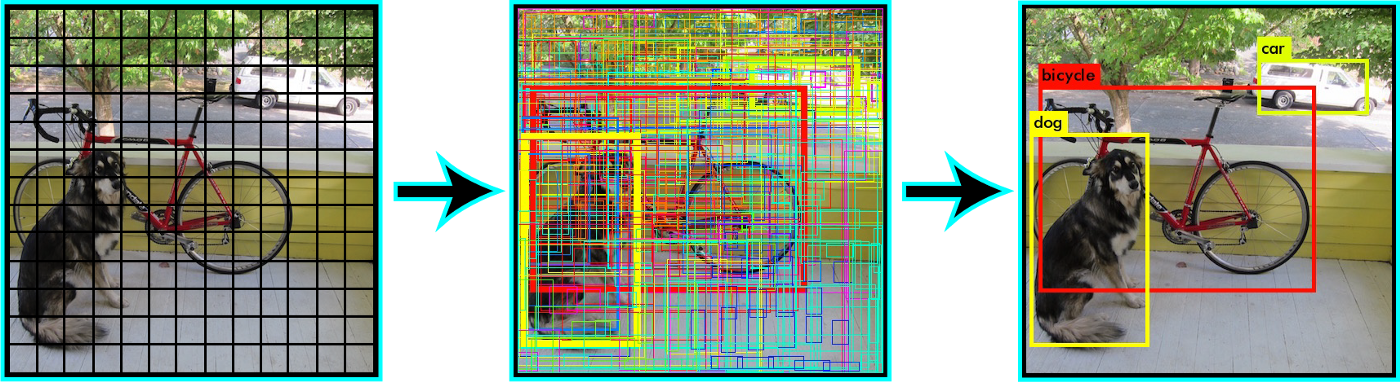
\includegraphics[width=\textwidth]{yolo}\vspace{1cm}


\section{Object Detection}

El Object Detection \cite{objectDetect} es un técnica de vision por ordenador que permite localizar imágenes y/o vídeos. Estos algoritmos se aprovechan del aprendizaje automático o del profundo 
con el objetivo de obtener resultados significativos, es decir, intentan replicar la inteligencia humana a la hora de reconcoer un objeto.